\documentclass{l3proj}

\begin{document}

\title{Team CSB - MyPHR Android Application}

\author{Jaskaran Bansal\\
        Holly Kirkham-Mowbray\\
        Giles Munn\\
        Charles Thomas}

\date{29 March 2018}

\maketitle
 
\begin{abstract}
Turner Syndrome is a genetic disorder affecting the growth and sexual development of approximately 1 in 2000 females. Those sufferers attending the Turner Transition Clinic at the Royal Hospital for Children, Glasgow, use a Patient Held Record to manage their medication and monitor their health.

This dissertation provides a case study of MyPHR, an Android mobile application developed for NHS Greater Glasgow and Clyde by four undergraduate Computing Science students at the University of Glasgow. The paper examines the software development process of creating a digital Patient Held Record, relating practices to existing research and reflecting on team experience.

\end{abstract}

\educationalconsent
\newpage

%============================================================================

\section{Introduction}
This paper is a case study dissertation of the Android mobile application MyPHR, developed at the University of Glasgow by Team CSB.

MyPHR was produced for NHS Greater Glasgow and Clyde and is designed for use by adolescent females with Turner Syndrome; it is a digital alternative to the Patient Held Record, a paper-based system for personal health monitoring and management that is currently provided to patients at the Turner Transition Clinic at the Royal Hospital for Children, Glasgow. MyPHR aims to match all functionalities of the current paper records on a more convenient, enjoyable, and discrete platform.

The purpose of this case study is to provide cumulative documentation of the production of MyPHR. It describes the project in great detail and closely examines the software development process this team undertook, reviewing the intentions and outcomes of this project and reflecting upon the events and experiences which defined the final result.

The dissertation is structured as follows:

\hyperref[sec:2]{Section 2} Case Study Background - a thorough description of the project context and concept, including:
\begin{itemize} 
    \item[--] \hyperref[sec:2.1]{2.1} Customer Organisation and Background
    \item[--] \hyperref[sec:2.2]{2.2} Project Motivation and Rationale
    \item[--] \hyperref[sec:2.3]{2.3} Initial Requirements and Objectives
    \item[--] \hyperref[sec:2.4]{2.4} Final Deliverable
\end{itemize}


\hyperref[sec:3]{Section 3} Reflection - a contemplative run through of the team's experience with the software development process, including:
\begin{itemize} 
    \item[--] \hyperref[sec:3.1]{3.1} Design Considerations
    \item[--] \hyperref[sec:3.2]{3.2} The Agile Development Process
    \item[--] \hyperref[sec:3.3]{3.3} Implementation
    \item[--] \hyperref[sec:3.4]{3.4} Process Improvement
    \item[--] \hyperref[sec:3.5]{3.5} Testing
    \item[--] \hyperref[sec:3.6]{3.6} Product Delivery
\end{itemize}

\hyperref[sec:4]{Section 4} Conclusion - a summarising look at the team's progression and achievements with this project, reflecting on what was learned as it came together.

%==============================================================================

\section{Case Study Background}\label {sec:2}
\subsection{Customer Organisation and Background}\label {sec:2.1}
NHS Greater Glasgow and Clyde (hereafter, NHSGGC) is a National Health Service board in West Central Scotland. This project was proposed by the Department of Paediatric Endocrinology at the Royal Hospital for Children, Glasgow (hereafter, RHC). Our primary contacts at the hospital were Consultant Paediatric Endocrinologist Dr. Avril Mason and Endocrine Nurse Specialist Ms. Teresa McBride; we also liaised with medical student Ms. Baryab Zahra.

The original, paper-based, Patient Held Record (hereafter, PHR) was devised by the Department of Paediatric Endocrinology to encourage adolescent girls attending the Turner Transition Clinic at the RHC to further their knowledge and awareness of their condition, and to promote self-advocacy in monitoring and managing it \cite{paperPHR}.

The proposed mobile application, outsourced to the University of Glasgow for development, is intended for the same user base as an equivalent alternative to the paper PHR. This user base consists of both Android and iOS mobile users, and so the proposal was divided for separate and independent development for these two platforms by our team and another, respectively.

Working with NHSGGC, the distinction in discipline between ourselves and our customer meant that establishing a good rapport and maintaining effective communication required some thoughtfulness. Care was taken throughout to avoid technical jargon which we may otherwise use and, similarly, a personal effort was made by all team members to understand Turner Syndrome and to get to grips with the associated medical terminologies used within the healthcare environment.

%==============================================================================

\subsection{Project Motivation and Rationale}\label {sec:2.2}
The project was proposed following a user study conducted at the Department of Paediatric Endocrinology Turner Transition Clinic. A focus group was held with patients at the clinic to assess the acceptability and user-friendliness of the current paper PHR, and returned a unanimous preference toward a mobile application alternative.

Providing a mobile application is intended to increase patient acceptance and engagement with the PHR system by making it available on a preferred platform. The increased participation expected from higher appeal aims to inspire greater success of the aforementioned goals - improving patients' knowledge and awareness of their condition, and strengthening their sense of responsibility over their health.

Achieving this will be instrumental in the greater goal of preparing those currently attending the clinic for their transition from paediatric to adult care.

%==============================================================================

\subsection{Initial Requirements and Objectives}\label {sec:2.3}
The key objectives for the project were outlined at our first meeting with NHSGGC; we used the MoSCoW method \cite{MoSCoW} to indicate requirement level.

The initial `must have' requirements for the project, which we guaranteed to deliver, were those core features and functionalities that the paper PHR currently provides:

\begin{itemize}
\item[--]Medication Management: the application must facilitate a record of the patient's current medications including a description, the prescribed dose and how often it should be taken.

\item[--]Appointment Management: the application must facilitate a record of the patient's past and upcoming clinic visits including the date, height and weight measurements taken at the clinic, and the means to note questions and other takeaways.

\item[--]Schedule of Investigations: the application must facilitate a record of past investigations such as blood tests, heart imaging, etc., and when they are due to be done again.

\item[--]Contact Information: the application must facilitate a record of contacts at the hospital and other medical staff which the patient may wish to contact in regard to their health.

\item[--]Offline Accessibility: the application must not require an internet connection to access the features; there is no public internet available at the hospital.

\item[--]Confidential and Secure: the application must be protected and private, the information contained may be sensitive and confidential.
\end{itemize}

The initial `should-have' requirements for the project, which were important but not vital, were those features made possible by moving to the mobile application platform:

\begin{itemize}
\item[--]Medication Reminders: the application should offer reminder notifications prompting the patient to take their medications.

\item[--]Medical Metrics: the application should provide meaningful statistical information about measurements taken regularly at the clinic, similar to the graphs and charts held on the hospital system.
\end{itemize}

The initial `could have' requirement for the project, which the customer found desirable but of lesser importance, was:

\begin{itemize}
\item[--]Calendar Element: the application could have a calendar view section, with medications and appointments marked.
\end{itemize}

There was one feature it was decided the application `won't have this time':

\begin{itemize}
\item[--]Parent and Doctor Accessibility: though briefly discussed, it was decided that the application would be for personal use by the patient only, in accordance with the desired push toward patient responsibility and independence in managing their health.
\end{itemize}

%==============================================================================

\subsection{Final Deliverable} \label{sec:2.4}
All of the `must have', `should have' and `could have' requirements proposed at the beginning of the project were successfully implemented by our team. Besides these initial objectives, there were also a small number of additional features which were proposed later in the project term.

The additional features which were achieved within the development period were:

\begin{itemize}
\item[--]Holiday Letter: at an early stage, another existing feature of the PHR was brought to our attention; the holiday letter describes the necessity for certain medications and medical equipment to be carried with the patient during travel and provides contact information for the appropriate staff at the hospital to corroborate the statement. As a simple feature, the addition was easily incorporated into the application.

\item[--]Appointment Reminders: in addition to the medication reminders described above, our team offered the customer notifications reminding the patient of upcoming appointments, as they are often scheduled far in advance. The customer believed this would be useful for users and the feature was implemented.

\item[--]Sick Day Tracking: our user study with a patient at the Turner Transition Clinic returned that a useful feature would be enabling days on the calendar to be marked as `sick days'; sick days are common for sufferers of Turner Syndrome, and the ability to see clearly when they have occurred would be valuable. The requirement was proposed at a later stage but it was simple to execute and was added during the final iteration.
\end{itemize}

There was one feature that was proposed during development that was not implemented in the end:

\begin{itemize}
\item[--]Hospital Directions: late in the project term, it was casually proposed that the app might provide mapped guidance to specified areas and rooms in the RHC. Due to the limited time remaining for development and the level of planning and interface rearrangement that would be required to execute the feature, we were forced to reject the idea. This was decided to ensure that the final deadline was met and that no other aspects of the application would suffer as a consequence of attempting more than was attainable.
\end{itemize}

%==============================================================================

\section{Reflection} \label{sec:3}

%==============================================================================

\subsection{Design Considerations} \label{sec:3.1}
Once the initial technical requirements had been established, work began designing an interface fit to accommodate the desired functionality. We chose a pink and purple colour scheme for our interface in reference to the Turner Syndrome Society, but selected a bolder hue to avoid direct association. This decision was founded in line with the sensitive nature of the application, as patients may be self-conscious of their condition and their peers may not be aware of their diagnosis.

This consideration carried importance throughout the design stage and a central quality of the application branding was, therefore, discretion. Owing to this we chose a name, MyPHR, and a logo, shown in Figure \ref{fig:logo_design}, which would be unassuming to those unfamiliar with the app. We found that working with such a restricted option pool was quite challenging, but ultimately inspired a great result.

\begin{figure}[ht]
  \centering
  
\includegraphics[width=50pt]{figures/logo_design.png}
  \caption{Logo Design}
  \label{fig:logo_design}
\end{figure}


\subsubsection{Initial Prototyping} \label{sec:3.1.1}
After thoughtfully examining the project requirements, we established that features fell into five main categories: contacts, medications, appointments, measurements, and the calendar. These formed the menu set for a quickly accessible bottom navigation bar. We then began to explore how individual pages would look. 

As we anticipated that requirements may change, we selected iterative interface prototyping as a great design technique to understand user needs and frequently return to the customer for valuable feedback on solid, presentable ideas \cite[p347]{psd-notes}. We also took an iterative approach with a range of app names and icons, until all were satisfied with the decision.

The first iterative prototyping stage asked all developers to propose a set of low-fidelity wireframes; beginning this way brought a large range of ideas to the table and encouraged discussion and a thoughtful decision. The design selected at this stage, a portion of which can be seen in Figure \ref{fig:initial_wireframes}, was favoured for its consistent and intuitive design, helping users to begin use immediately, not subject to any learning curve. This was an important factor given our goal to improve acceptability.

From this rough wireframe set, the next iteration was to create higher-fidelity UI mock-ups, a portion of which can be seen in Figure \ref{fig:final_wireframes}, which we could bring to the customer for their opinion. We received great feedback for these designs, with just one semantic tweak proposed, allowing us to begin implementation of our vision. 

\begin{figure}[ht]
  \centering
  \begin{minipage}[b]{0.48\textwidth}
    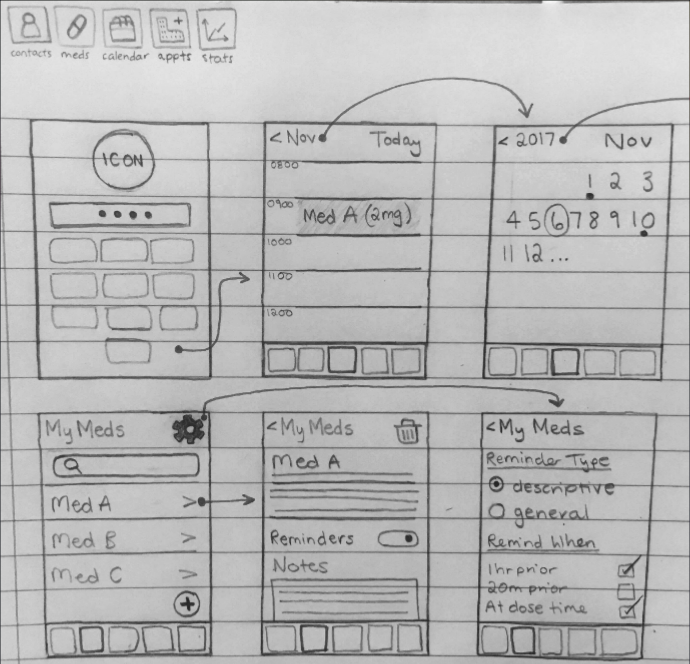
\includegraphics[width=\textwidth]{figures/initial_wireframes.png}
    \caption{Initial Design Draft}
    \label{fig:initial_wireframes}
  \end{minipage}
  \hfill
  \begin{minipage}[b]{0.48\textwidth}
    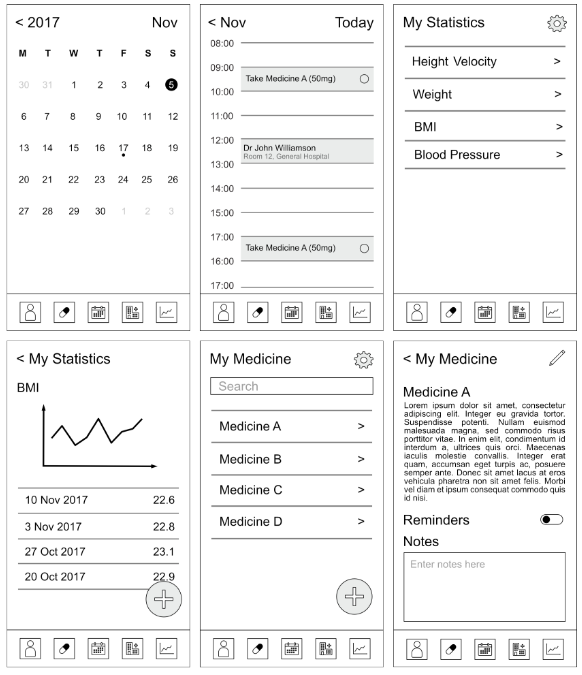
\includegraphics[width=\textwidth]{figures/final_wireframes.png}
    \caption{User Interface Mock-ups}
    \label{fig:final_wireframes}
  \end{minipage}
\end{figure}


\subsubsection{Final Design} \label{sec:3.1.2}
As development of the application advanced, its design was continuously iterated upon and refined for purpose. Referring to Google’s Material Design guidelines \cite{material-design} supported design decisions throughout, helping us create an interface in line with Android standards and so provide familiarity for users. A portion of the final design can be seen in Figure \ref{fig:final_design}.

\begin{figure}[ht]
  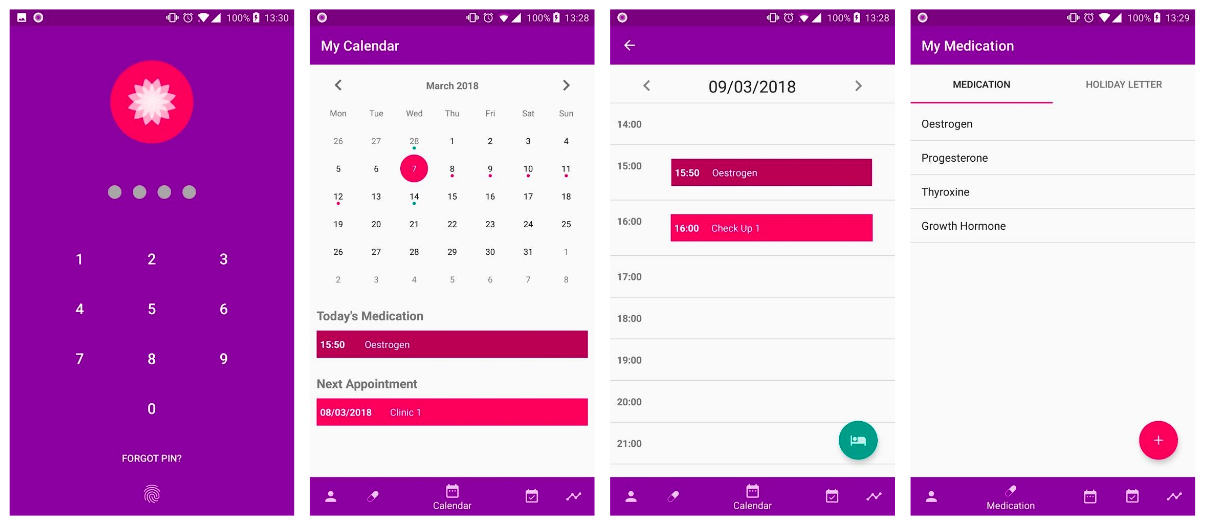
\includegraphics[width=\linewidth]{figures/final_design.png}
  \caption{Final Design}
  \label{fig:final_design}
\end{figure}

As anticipated, the interface had to be altered to satisfy additional requirements as they emerged - tabs were introduced to accommodate the holiday letter and the structure was replicated across appointments and measurements, too, to streamline and separate features. The calendar was also adapted to incorporate a floating action button to mark sick days.

Some design aspects were also removed for even smoother interaction - search bars were identified as extraneous due to the likely low number of list items, and settings pages were scrapped and incorporated into details fragments to allow for reminder options specific to individual medications and appointments.

We had to make a significant number of changes like this as the project progressed and many owed to oversights made at the initial design stages. Some features, such as user input screens, hadn't been given enough attention during prototyping, and some others were missed altogether. When implementing the login activity, we realised that our designs thus far had not considered a coping mechanism for a forgotten PIN; after some discussion, we introduced security questions at set-up and a forgotten PIN section, accessible from the login page, but this was a tricky problem.

Reflecting on our design process, we believe that an iterative approach brought us to an excellent result. Continuously reassessing our decisions helped us to identify useless features and incorporate new project requirements, and we are happy with the outcome. That said, we regret that so much was overlooked initially, and the ongoing changes and rearrangement which we suffered as a result. For future projects, we learned the value of planning and investing greater time and thought into earlier prototypes to get things right the first time.

%==============================================================================

\subsection{The Agile Development Process} \label{sec:3.2}
Our team took an agile approach to development. Agile is a software development process under which requirements evolve and delivery is incremental; the Agile methodology values individuals over tools and working software over design and documentation \cite{AgileMain}. The Agile approach suited our small team size well, and accommodated flexible software engineering by which we could respond to evolving customer and developer needs. Unanimously, we would certainly follow Agile practices again.


\subsubsection{User Stories and Scenarios} \label{sec:3.2.1}
At the project start, we created a pool of user stories and scenarios to ensure a common set of assumptions among developers and create a series of references to return to throughout and reconfirm user needs.

Creating user stories \cite[p254]{psd-notes} is a technique for succinctly expressing user requirements that is common in Agile development frameworks such as XP \cite{extreme}. Initially, we used user stories to incite meaningful discussion about our project requirements from the personal perspective of our users. Throughout development, we referred back to them to ensure we were meeting their needs both technically and as real people relying on our application. 

We created user scenarios \cite{userscenarios} to draw a wider focus, not only on individual features to achieve, but on the application as a whole and whether it caters fully for those wishing to incorporate MyPHR into their healthcare regimen and life. Through user scenarios, we began to understand what our users are looking for from our mobile application and what motivations and concerns they have about their current situation that our product can improve.

While designing for a user base to which none of us can personally relate, user stories and scenarios were invaluable in understanding user needs beyond the technical, and ensuring that we kept them in mind throughout development. Assessing our final product, we believe the practice was extremely worthwhile in keeping us focused on both functional requirements and bigger-picture user needs. Exploring our user this way is how we came to offer tailored reminder options to control the explicitness of notifications - this was not a requirement requested by our customer, but by thoroughly understanding our user we knew how valuable this option would be.


\subsubsection{Team Organisation} \label{sec:3.2.2}
From the Agile Manifesto: ``The best architectures, requirements, and designs emerge from self-organising teams." \cite{AgileManifesto} Our team adopted the self-organising model. As a group of highly motivated individuals, we decided that this dynamic and adaptive team configuration would be the most natural and successful for us. Looking at what we achieved, we completely stand by this decision and thoroughly enjoyed working in this way. 

Kaltenecker and Hundermark describe the self-organising team as characterised by ``distributed control, continuous adaptation, emergent structure, feedback and resilience" \cite{SOTeams}. The self-organising team means collective goals and individual responsibility; requirements are dynamic and contributions are self-governed. 

We chose self-organising as it allowed for a dynamic and reactive group of tasks to be continuously generated and resolved by any developer. The model was chosen over a more Mechanistic \cite{mechanistic} team structure, with role assignments and a strict compartmentalisation of work, as it accounted for uncertainties around the difficulty level of executing features we had no previous experience with - such as notifications - and also in anticipation that many areas of the project would fluctuate some in weight and complexity as requirements changed.

Though ready to reassess if moving too slowly, we found that self-organising proved extremely motivating, satisfying, and successful. The model worked for us but relied on a skilled and proactive development team propelled by individual enthusiasm and a compelling goal. Without strict responsibilities, careful communication was required to ensure that all project targets would be met; as discussed in \hyperref[sec:3.2.5]{Section 3.2.5}, thoughtful issue tracking to this end was accommodated through GitLab. 

Evidenced by the timely completion of project goals and delivery of the final product, we believe that our team was highly successful under this structure. We endorse that this was because of the  motivated individuals involved and in future projects, with a similarly enthusiastic team, we would all certainly advocate self-organising. 


\subsubsection{Code Ownership and Review} \label{sec:3.2.3}
Our team adopted a weak code ownership scheme for development \cite{CodeOwnership}. Weak code ownership has individual developers command loosely drawn areas of personal responsibility, assumed of one's own volition, while giving all the freedom to make changes within the domain of others. We identified this model as suitable for the nature of our project, where a loose compartmentalisation of tasks would be possible, but features were too intertwined to separate strictly.

We believe that this model worked excellently for us. Weak code ownership meant individuals developed a deep understanding and expertise over their personal scope, while also encouraging a working comprehension of that outwith their domain and allowing transcending features to be implemented by a single developer without extensive permissions gathering. To support the arrangement, we introduced software inspections and all subsequent merge requests to master were directed through another developer for code review and approval.

Cohen et al. assert that the primary benefit of peer code review is early bug detection \cite[p9-16]{CodeReview}. This was not our team's emphasis when introducing the practice and, as explored further in \hyperref[sec:3.4.4]{Section 3.4.4}, we had little success in that regard as a result.

The primary reason that our team introduced code reviews was to improve code comprehension and so support our weak code ownership scheme, by giving developers the confidence to work throughout the codebase when necessary. The practice was useful when features were interconnected - for example, it helped the developer managing user input understand how the developer in charge of plotting medical metrics expected to receive their data, e.g. dates in the Java Date format. 

We appreciate how code reviews aided our code comprehension but, on reflection, a technique such as code walkthroughs \cite{Walkthroughs} may have been better at achieving both this and bug detection too. The writer may be more likely to catch errors when explaining their own code than having a reviewer try to both understand the code and detect errors too.


\subsubsection{Pair Programming} \label{sec:3.2.4}
Pair programming is an Agile technique in which two developers work together at one machine; one programmer, the pilot, takes control writing code while another, the navigator, watches and identifies errors and shortcomings as they arise \cite[p95]{psd-notes}.

We introduced pair programming at the point of database implementation; data is pulled from the database in almost every class, so an understanding was crucial for all team members. To this end we had been using code reviews, but they were becoming repetitive and developers were getting complacent as a result; we put two minds on the task and believe this ended up being key to getting the database right first time. We learned that it is crucial in development to recognise when things that were once successful have stopped working and to react accordingly.

Following the success of the technique in this case, we tried it again when work began implementing measurement graphs. In this case, however, we found that the practice actually hindered production and we suffered `too many cooks' as developers clashed with differing personal preferences about which libraries and methods to employ. We learned that pair programming may be less effective in situations where there is considerable room for creative freedom and not one correct answer - after one session, we returned control to a single developer and inspection by code review. 

Though not a strong focus of our development process, we would employ pair programming again to tackle tasks which would benefit from shared developer knowledge but where there is a limited range of solutions. Where decisions can be more subjective and personal preferences come in to play, however, we found it only hindered the development process, and we would choose another inspection technique. 


\subsubsection{Issue Tracking} \label{sec:3.2.5}
With a lack of shared physical space during development, accessible issue tracking was accommodated through GitLab - this also provided automated project metrics and an easy visualisation of progress throughout development \cite[p277]{psd-notes}.

Assignment of issues was predominantly voluntary and though, on occasion, an undesirable task would linger and require discussion, generally this arrangement was extremely effective and allowed personal strengths and passions to be utilised. Team members were also free to assign issues to other developers where appropriate; should a bug or some problem be identified under another developer’s scope, the author could be notified to deal with the issue, as the most knowledgeable over that code. 

Careful issue tracking also aided effective time-keeping which was crucial for a short-term project such as this. Coupling of issues with project iterations and application of specific due dates ensured continuous progression, with incremental deadlines propelling development.

Unanimously our team would use this issue tracking technique again. The flexible arrangement worked excellently with our self-organising structure and weak code ownership scheme, and should we work on similar projects in the future we would track progress this way again.

%==============================================================================

\subsection{Implementation} \label{sec:3.3}
Implementation began in iteration two and a range of technologies were selected and introduced for development. Throughout the process, careful attention was payed to both the front and back end of the application and thoughtful planning and decision making ensured a happy cohesion between the two. 

The diagram shown below in Figure \ref{fig:architecture} represents the architecture model. This model was designed such that all Activities and Fragments within the application would have a direct connection to the database so they could display any required data without needing to pass through any complicated channels.

\begin{figure}[ht]
  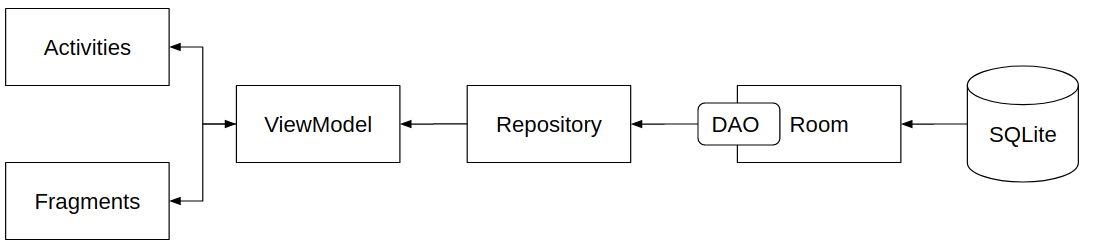
\includegraphics[width=\linewidth]{figures/architecture.png}
  \caption{Architecture Model}
  \label{fig:architecture}
\end{figure}

As described in \hyperref[sec:3.1.2]{Section 3.1.2}, changing requirements presented design challenges when implementing the front end of the application, but a number of technical challenges also arose. In the back end, a strong existing knowledge of database structure needed translation into the application itself, and it too was tweaked as development progressed due to minor initial oversights and changing requirements. 


\subsubsection{Technologies Used} \label{sec:3.3.1}
Functional and design requirements established, attentions were turned to determining which technologies would best implement our vision. 

It was quickly established that we would develop using the Android Studio IDE; the team unanimously agreed that the purpose-built environment would be most suitable. Android Studio was favoured for its many desirable features such as drag-and-drop UI design and integration of the Gradle build tool. The selection also meant avoiding extraneous proprietary IDE files and, perhaps most compellingly, allowed for instant testing by running the application on an Android device or via on-screen emulator.

Not all developers had previous experience with Android Studio when development began, meaning a stronger learning curve for half of the team. At the project start, the use of pair programming and code walkthroughs \cite{Walkthroughs} of the main application set-up allowed more experienced team members to share their knowledge with those just starting out. These developers found that they were fully confident developing in the IDE after a few weeks, and this was supported by the wealth of documentation and community support owing to the popularity of the software.

Another fundamental decision was determining whether to code in Java or in the newly developed Kotlin programming language. Kotlin was considered as a promising new language with more concise code and other attractive attributes, but Java was ultimately chosen for developer familiarity - the ability to begin work immediately and confidently outweighed the benefits of learning a new language.

Incremental development was assisted by Git, using a virtual machine hosted GitLab repository to house code. This provided crucial tools such as use of feature branches, the ability to rollback mistakes, and continuous backups. Git was a familiar technology for most of the team but one developer had no previous experience with the system. For them, the learning curve was steep but assistance from other team members at the initial stages helped them greatly and, again, they were confident contributing through Git after a few weeks.

The majority of the application was written using built-in Java and Android libraries, however a couple of external libraries were also pulled in to execute more complex features. The first of these was the login screen - to assist in achieving the envisaged design, with custom PIN keyboard and input indicator dots, an external library, PinLockView, for this purpose was used \cite{pinlock}. 

The second instance was the use of GraphView \cite{graph-view} to achieve the dynamic and responsive graphs in the measurements section. GraphView is an open-source graph plotting library which allowed for graphs which update instantly as users edit data points, scroll to display historical data, and accommodate the use of the Java Date type for x-axis scales. External libraries eased the workload when implementing tricky features and were of great use to the team.

More technologies were introduced to assist testing - the use of Espresso \cite{espresso} greatly increased the efficiency and effectiveness of user interface testing, as discussed in \hyperref[sec:3.5.1]{Section 3.5.1}, and JaCoCo \cite{jacoco} allowed us to create useful code coverage reports, explained in more detail in \hyperref[sec:3.5.2]{Section 3.5.2}.


\subsubsection{Front-end Implementation} \label{sec:3.3.2}
The front-end of MyPHR was extremely important, with the presentation layer carrying a large portion of application function. Given the project goals of increased acceptance and engagement with the PHR system, a significant amount of thought and time was invested in the appeal and usability of the application interface. Thoughtful features such as useful feedback, in the form of live input error checking, and forcing functions, in the form of lock-ins \cite{lock-ins} upon data deletion request, made for an interface that supports and guides interaction.

The application front-end was based in XML layout files, and features were accessed and brought to life programmatically from the main code. The team found this separation of concerns to be very useful, especially when dealing with trickier screens, such as the login activity, which required multiple custom layouts to be defined for different device screen sizes.

A significant challenge we faced when developing the front-end was an issue with the calendar; upon scrolling the day view, appointments and medications scheduled for that day would begin to multiply and appear in other time slots. After extensive research into the problem, the cause was identified - to display events, the developer had employed the same list structure used repeatedly throughout the application, but in this case it was not actually fit for purpose. The consequential restructuring took significant developer time but had the calendar functioning as required. Setbacks like this were perhaps the most frustrating, where work had to be repeated due to initial oversights; developers learned that prior planning and research into the best way to accomplish a task is crucial, as simply relying on techniques one is comfortable with can result in an inadequate solution and more work in the long run.

\subsubsection{Back-end Implementation} \label{sec:3.3.3}
The database back-end of MyPHR was anticipated to be easy enough due to the small quantity of simplistic data involved in the application, and so its implementation was left until a fair amount of the front-end had been established. We used the SQL Database Modeler tool \cite{sqldbm} to design the database schema, and, as expected, it was quite simple to create - only one relationship was required relating a single Statistic (the type) to many Statistic Values (the measurements).

There were many technologies considered to build the database, such as Sugar or GreenDao, but Android's own Room Persistence Library \cite{room} was selected. Room offers a high-level interface over SQLite, a powerful database management tool. We chose Room to avoid reliance on third-party libraries, and as it allowed us to fully concentrate on the higher-level components of the database - queries and entities -  avoiding additional set-up and boilerplate code. As the application was to be completely self-contained and local on the user’s device, Room would be very capable of performing the data management required.

The database required a simple redesign on one occasion to incorporate the new Sick Day Management feature introduced at our user study; the final database model including the new entity is shown in Figure \ref{fig:final_db}.

It is worth noting that reminder options, on the other hand, were already included in individual instances of the medication/appointment entities in the initial database model - resolution of design uncertainties such as the use of settings pages \textit{before} back-end implementation began was the benefit of leaving it to a later stage in development, as many resultant rearrangements of the database were avoided. We would only advocate this decision again, however, with similarly simplistic projects. 

\begin{figure}[ht]
  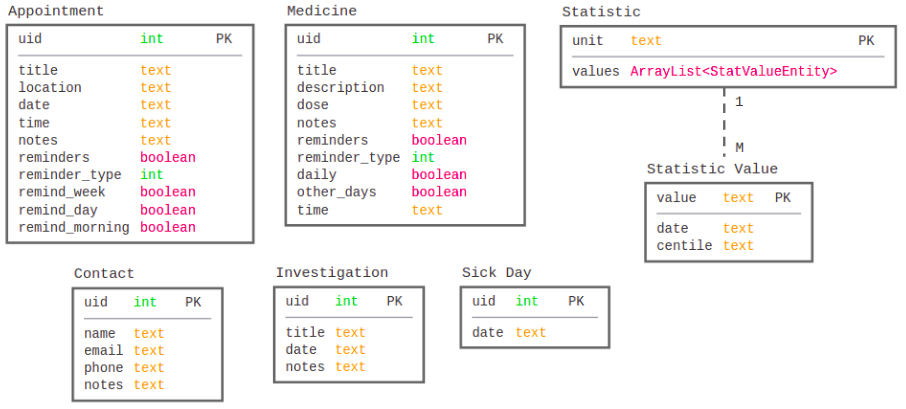
\includegraphics[width=\linewidth]{figures/final_db.png}
  \caption{Final Database Model}
  \label{fig:final_db}
\end{figure}

We should also recognise the disparity between naming conventions in the back-end compared to the sections as the user knows them. Late in the development of MyPHR, the section formerly known as `medicine' was changed to `medication', and that known as `statistics' was changed to `measurements' - these were both deemed more accurate descriptions, but we regret that the update was not carried through the codebase also. Unfortunately this inconsistency could cause confusion and impact software maintainability in the future but, in line with Agile principles, we prioritised working software over the cleanest code. Our team, once again, regretted not being more thoughtful early on and confirming these decisions before the codebase got too large to feasibly change - a lesson we will certainly carry forward to future projects.

A significant issue was caught during interface testing where different appointments of the same title would take users to the same details page. The error occurred due to an oversight where the details page would query the database by non-unique appointment title, rather than the auto-generated UID primary key. Once the problem was found it was swiftly corrected, and all other sections were scoured to ensure queries were executed correctly. 

This discovery uncovered an issue that had been creeping up on our team - as the project drew on, developers were slipping in the thoroughness of code reviews. As discussed in \hyperref[sec:3.4.4]{Section 3.4.4}, merge sizes were reduced in an attempt to improve the process, and more time was also invested in other inspection techniques, such as pair programming. The team struggled with maintaining effective code inspection, and in the future we would endorse using multiple techniques to avoid tedium and support successful reviews. 

Database aside, a challenge also arose in accommodating different Android versions. Though initially catering for newer API levels only, we decided upon reviewing Google’s statistics \cite{dashboards} that we should support versions as far back as Android 5.0, as over a fifth of users still run these older versions. This change meant a fair amount of additional work to ensure features such as notifications and fingerprint scanning accounted for API level and were disabled when necessary. Whilst catering for this group was an additional expense of time and efforts, our team recognised that backwards-compatibility is valuable, and much of our user base may rely on such considerations. We believe that in software development it is crucial not to exclude certain user groups if it can be avoided, and we certainly didn't want any patients missing out due to owning an older device. 

%==============================================================================

\subsection{Process Improvement} \label{sec:3.4}
From the Agile Manifesto: ``at regular intervals, the team reflects on how to become more effective, then tunes and adjusts its behaviour accordingly."\cite{AgileManifesto} It was crucial for sustaining steady progression and team success that we take a reflective approach throughout development and responded dynamically to continuously improve.


\subsubsection{Retrospectives} \label{sec:3.4.1}
Throughout the project life cycle, the development process was regularly evaluated and adjusted by conducting regular retrospective meetings and acting on the outcomes. Following each customer meeting at the conclusion of a project iteration, a reflective examination of the sprint was performed by our team to determine how we could improve our organisation and methodology during the next iteration. 

Initially we trialled two different retrospective techniques to determine the most suitable method for eliciting meaningful takeaways from each sprint. We first explored the Sailboat method \cite[p21]{Sailboat}; the Sailboat method involves metaphorically representing process goals, risks, helps and hindrances as islands, rocks, anchors and clouds, respectively. We found that this technique did not inspire a quality analysis by our team, resolving that it was too obscure and did not represent enough of a call to action looking forward.

The second retrospective technique which we trialled, and selected, was Start, Stop, Continue \cite{SSC}; Start, Stop, Continue is an action-oriented method which identifies behaviours and techniques from the previous iteration which were:

\begin{itemize}
    \item[--]missing or lacking and should be applied in the next sprint (`start');
    \item[--]redundant or damaging and should be left behind moving forward (`stop');
    \item[--]useful or successful and should be maintained during the next sprint (`continue').
\end{itemize}

The use of retrospectives was new for all team members, and we valued selecting the right method for us. Using these categorisations to form clearly defined lists of actions, the team made valuable assessments about the development process throughout and frequently set clear goals by which it should improve. 


\subsubsection{Iteration One}\label{sec:3.4.2}
Iteration one was the design phase and a happy reception of the UI mock-ups we presented left us with little but praise from the customer meeting; the associated retrospective drew a focus on improving customer interaction and meeting organisation.

We recognised that during the first sprint we had established a good team rapport and that this was apparent in front of our customer. What lacked was quality takeaways and direction to inform our next steps, as the acceptance of our prototypes meant no issues were generated from the customer side. We learned the importance of preparation, and we resolved to do more in future to elicit information.

We also found our meeting notes were not as cohesive and complete as we would like; we identified that having one note-taker, also engaged in conversation, was not working and we resolved to appoint two designated note-takers and two designated communicators from then forward - a technique we would endorse in the future. 


\subsubsection{Iteration Two} \label{sec:3.4.3}
Iteration two was the start of implementation and in our customer meeting we saw a marked improvement following our strategy change; the retrospective drew a focus on team organisation and how we can better communicate and collaborate together.

As work began in our GitLab repository, some overlap occurred in what was produced, difficult merge requests arose, and we struggled to understand each other's work; we resolved to make better use of issue assignment, branching, and to improve code commenting. We learned that collaboration requires thoughtfulness, and that careful consideration for other developers is crucial for smooth operation.

We also identified communication as a cause of team confusion. Communication was scattered across multiple platforms and often involved just a subset of the team; we resolved to move all communication to one platform to combat the disorder.


\subsubsection{Iteration Three} \label{sec:3.4.4}
Iteration three saw development in full swing and we found we had a better command of individual responsibilities following the last sprint; the retrospective drew a focus on improving the technical process as progression accelerated and the codebase grew.

As we pressed on, complicated merge requests arose owing to large contributions of many hundreds of lines. Code reviews, introduced at the start of the sprint, became increasingly laborious and difficult as merges were extensive. Developers were getting sloppy and bugs slipped through to master, so we resolved to ease the process by merging less code, more frequently, and incorporating alternative inspection techniques to reduce tedium. The experience demonstrated the importance of process improvement techniques to identify when processes stop working effectively.

This retrospective also took a strong look forward. Though progressing steadily, we wanted to define clear deadlines for the remainder of the project term, and begin the accompanying case study with ample time. 


\subsubsection{Iteration Four} \label{sec:3.4.5}
By iteration four, we had worked out a process that was really working to get the most out of our team, and near-all functionality of MyPHR was implemented in time for our final customer meeting. The retrospective focused on directing a greater share of attention to the case study, in tandem with refinement of our final product. 

%==============================================================================

\subsection{Testing} \label{sec:3.5}
To our team, Agile testing meant a focus on risk-based prioritisation and efficiency through automation. We used incremental testing to keep testing up to date with the progression of our project and ensure quick detection of problems when they arise. Incremental testing was favoured for its flexibility over other methods such as the Waterfall model \cite{Waterfall}, which is less suitable for an iterative development process. 


\subsubsection{Local and Instrumented Unit Testing} \label{sec:3.5.1}
There are two main types of unit testing within Android development - local and instrumented \cite{unit-tests}. Local unit tests operate on methods which do not require UI elements or the building of the application; they run quickly and test the logic of small functionality. Oppositely, instrumented unit tests operate on methods which \textit{do} rely on UI elements and running them requires the application to be built.

As MyPHR is very interface focused, there were far more areas where instrumented unit tests were beneficial than where local unit tests were effective. Just a small number of local unit tests were implemented on those methods which do not involve UI, such as correct calculation of when `every-other-day' medications should be taken.

Instrumented unit tests were implemented to guarantee interface elements performed as expected; they covered features such as correct database builds, accesses and updates.  We used the Espresso testing framework \cite{espresso} to create UI tests. Espresso provides an API which can be used to spoof interactions and state expectations without the need for extraneous boilerplate code - this aided the efficiency of test creation immensely. In conjunction, Android Studio provides the Espresso Test Recorder \cite{espresso-recorder}, which allows you to simply record interactions with the application and add assertions throughout; the tool was incredibly useful when creating larger tests for features such as the forgotten PIN section - a test to set a PIN and security questions then reset the former using the latter could be implemented quickly and efficiently.


\subsubsection{Code Coverage} \label{sec:3.5.2}
We utilised the JaCoCo code coverage library \cite{jacoco} to measure the code coverage of our unit tests. We chose JaCoCo as, unlike Android Studio's built in tool, it covered instrumented unit tests as well as local. Compared to other external tools, such as Emma \cite{Emma}, we chose JaCoCo for its quality documentation and useful code coverage reports, which clearly show which lines and branches are covered by testing, and which are not. The highest-level of the code coverage report is shown in Figure \ref{fig:code-coverage}.

\begin{figure}[ht]
  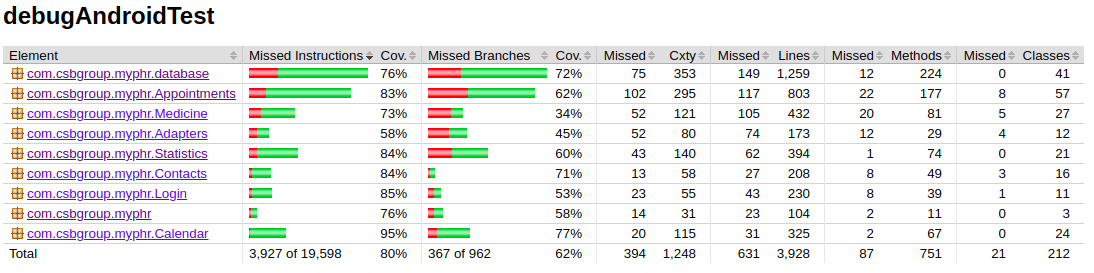
\includegraphics[width=\linewidth]{figures/code_coverage.png}
  \caption{Code Coverage Report}
  \label{fig:code-coverage}
\end{figure}

From these reports we found that we achieved a statement coverage of 80\% and a branch coverage of 62\%. Our coverage was not 100\% as we decided not to spend time implementing tests with little benefit just to boost this number, we prioritised important application functionality and are confident our testing was amply thorough.


\subsubsection{Continuous Integration} \label{sec:3.5.3}
We used the GitLab Continuous Integration (hereafter, CI) tool \cite{gitlab-ci} throughout development to build and test the current version of our application on all branches. CI was incorporated at merge time to ensure minimal disruption when incorporating feature branches; the merge would be blocked should the build or tests fail, identifying issues within committed code and ensuring the master version remained functional.

While local unit tests were integrated smoothly into our CI process, attempting to incorporate instrumented unit tests was a struggle. Instrumented unit tests require the use of a physical device or emulator, and an inability to enable hardware acceleration on our CI OpenStack instance inhibited them from being run at merge time. Though not an ideal situation, we resolved not to sink excessive time into overcoming the issue, as the tests could still be run outside of the CI environment and so was not a threat to the integrity of our app. We learned during this project that prioritisation is imperative to achieving what is most important, and we advocate that a similar sensibility throughout was instrumental in meeting all of our project requirements. 


\subsubsection{User Testing} \label{sec:3.5.4}
While our team worked continuously to explore all corners of possible user interaction and uncover any shortcomings and bugs, a valuable assessment of the suitability of MyPHR could only come from those within the target demographic. Unfortunately, due to the sensitive nature of the project and the young age of the users, conducting a complete and thorough user study was not possible.

We were thankful, however, that our customer managed to arrange for us a meeting with one patient of theirs at the RHC. We prepared a short questionnaire to elicit feedback from the participant which aimed to assess the attractiveness, usability and suitability of MyPHR for their needs. The response was extremely positive and an invaluable suggestion we received was to enable sick days to be marked on the calendar, an insight we couldn't have gleamed from anywhere else.

While we recognise that one participant is not a thoroughly revealing user study, we were happy to hear that the individual found our design worked for them and that they were excited to begin using the system, and we believe the sick day idea alone made it a worthwhile exercise.

%==============================================================================

\subsection{Product Delivery} \label{sec:3.6}
The final project milestone was delivering the finished product to our customer, and making MyPHR accessible for patients to begin using. NHSGGC expressed that we should take care of the latter task too, as they would not know how to take the codebase and make the application accessible themselves.


\subsubsection{Deployment to User} \label{sec:3.6.1}
Two methods for deployment were taken under consideration - an official release to the Google Play Store, or the distribution of the compiled APK to be `sideloaded' by each user. Sideloading was considered for its direct delivery to patients, avoiding public accessibility of the software (thus supporting discretion and privacy), and also for lack of associated cost. Despite these merits, the final decision was to deploy MyPHR officially on the Play Store. Following discussion with NHSGGC, the ease of downloading from the store was deemed the most valuable consideration, especially given the young and not necessarily technically proficient target demographic. 

Deployment on the Play Store was also advantageous for \textit{us}, as the developer console provides useful usage statistics and crash reports. Furthermore, should necessary updates or fixes emerge down the line, changes can easily be pushed as an update to the app - far preferable to repeating the sideloading process.


\subsubsection{Delivery to Customer} \label{sec:3.6.2}
We created a ZIP archive of the final application codebase for delivery to our customer, NHSGGC. Along with the codebase, we provided accompanying code documentation via Javadoc. Javadoc generates compiled documentation from specially formatted commenting in Java source code \cite{Javadoc}. We used Javadoc commenting to explain methods defined throughout our program and ensure a high level of code readability and maintainability.

Though we adopted Agile development over more document-driven methodologies, we believe using this formal documentation method encouraged consciousness and completeness from our team when developing, and that the resulting software is more understandable and maintainable for potential future use.

%==============================================================================

\section{Conclusion} \label{sec:4}
Developing a complete piece of software for a real client to put to real use was a new experience for our team, and as such we were enthused and determined to do our best work. Now, at the project conclusion, we can say that we are proud of our final product, and that we achieved what our customer expected and our users deserve.

The first thing we gained from the creation of MyPHR was a great deal of technical skill. As discussed, team members began with varying experience levels, but by delivery every developer felt confident in the work we were doing, and comfortable navigating a project of such scale.

Even more so we gained a wealth of knowledge about effective teamwork and collaborative software engineering. From our time in development, and from reflecting carefully on those experiences in the production of this case study, we can identify three most salient takeaways which we learned about successful software development.

The first lesson we will take forward is the value of prioritisation. As discussed within, we made tough decisions in the face of unexpected changes (such as altering section names) and during testing which sacrificed certain standards in our project. We took these minor hits in pursuit of our greater goals for the project, and we are extremely proud to have met all of our customer's formal requirements in sufficient time and to a high standard. 

The second key lesson which our experience highlighted was the importance of process improvement techniques. Evaluating our practices and, most prominently, recognising when a method which once worked no longer suited the process circumstances was crucial. We saw this in full effect with the steady deterioration of our code review process, and we attribute much of our success to how our operation benefitted from revisions made to combat these issues. 

The final lesson, which we found came up again and again, was the value of careful planning and investment of time early on to avoid additional or repeated work down the line. This theme recurs through our discussions of design, of calendar implementation, and again with section naming. Our team all felt the effects of `under-thinking' and would advocate a greater stress on planning in the future. 

While, for the most part, development was smooth and enjoyable, we learned a lot about the software engineering process and gained many valuable takeaways. We will carry forward the technical knowledge we gained and lessons we learned in the importance of proper software development practices, and feel confident in our abilities when endeavoring future projects. 

%==============================================================================

\newpage
\bibliographystyle{plain}
\bibliography{dissertation}

\end{document}